%% beamerthemeImperialPoster v1.0 2016/10/01
%% Beamer poster theme created for Imperial College by LianTze Lim (Overleaf)
%% LICENSE: LPPL 1.3
%%
%% This is the example poster demonstrating use
%% of the Imperial College Beamer Poster Theme
\documentclass[xcolor={table}]{beamer}
%% Possible paper sizes: a0, a0b, a1, a2, a3, a4 (although Imperial College posters are usually A0 or A1).
%% Possible orientations: portrait, landscape
%% Font sizes can be changed using the scale option.
\usepackage[size=a0,orientation=portrait,scale=1.55]{beamerposter}
\usepackage{wrapfig}

\usetheme{ImperialPoster}

%% Four available colour themes
\usecolortheme{ImperialWhite} % Default
% \usecolortheme{ImperialLightBlue}
% \usecolortheme{ImperialDarkBlue}
% \usecolortheme{ImperialBlack}

\title{The Principled Violation of Policy: Norm Flexibilization in Open Self-Organising Systems}


\author{David Burth Kurka and Jeremy Pitt}

\institute{Department of Electrical and Electronic Engineering, Imperial College London}

% \addbibresource{sample.bib}


\begin{document}
\begin{frame}[fragile=singleslide,t]\centering

\maketitle

\begin{columns}[T]

%%%% First Column
\begin{column}{.47\textwidth}

\begin{block}{Motivation}

\begin{itemize}

\item \textbf{Rules and norms} in open systems attempt to guarantee its well functioning and prevent selfish (e.g.\ free-riding) or unsustainable (e.g.\ tragedy of the commons) behaviour. 
\item \textbf{Sanctioning} structures prevent and punish non-compliance enforcing conformity.
%
\item To what extent sanctioning strategies really have \textbf{beneficial effects} in socio-technical systems?
\item In what extent full norm compliance is a desirable outcome and at what \textbf{cost}?
%
\end{itemize}

\end{block}


\begin{block}{Layers of Society Simulation}
\begin{figure}
  \centering
  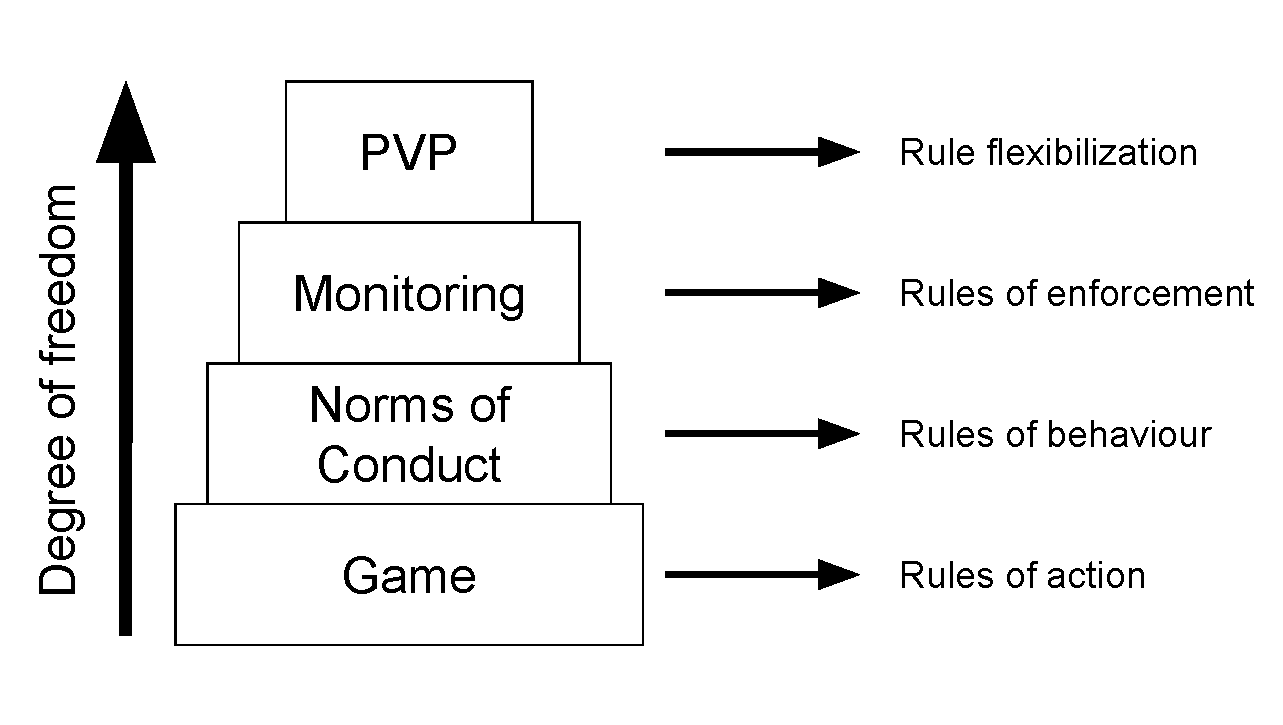
\includegraphics[width=0.8\linewidth]{img/ruleslayers.pdf} 
%  \caption{Layers of rules involved in the design of CAS simulations.}
  \label{fig:rules}
\end{figure}


% \begin{block}{Principled Violation of Policy}

\textbf{Principled Violation of Policy} -
\emph{The active and
intentional decision of an agent of not applying a policy to which it is entitled.}


\end{block}


\begin{block}{Setup: $LPG'$ with sanctions and forgiveness}
\begin{figure}
  \centering
  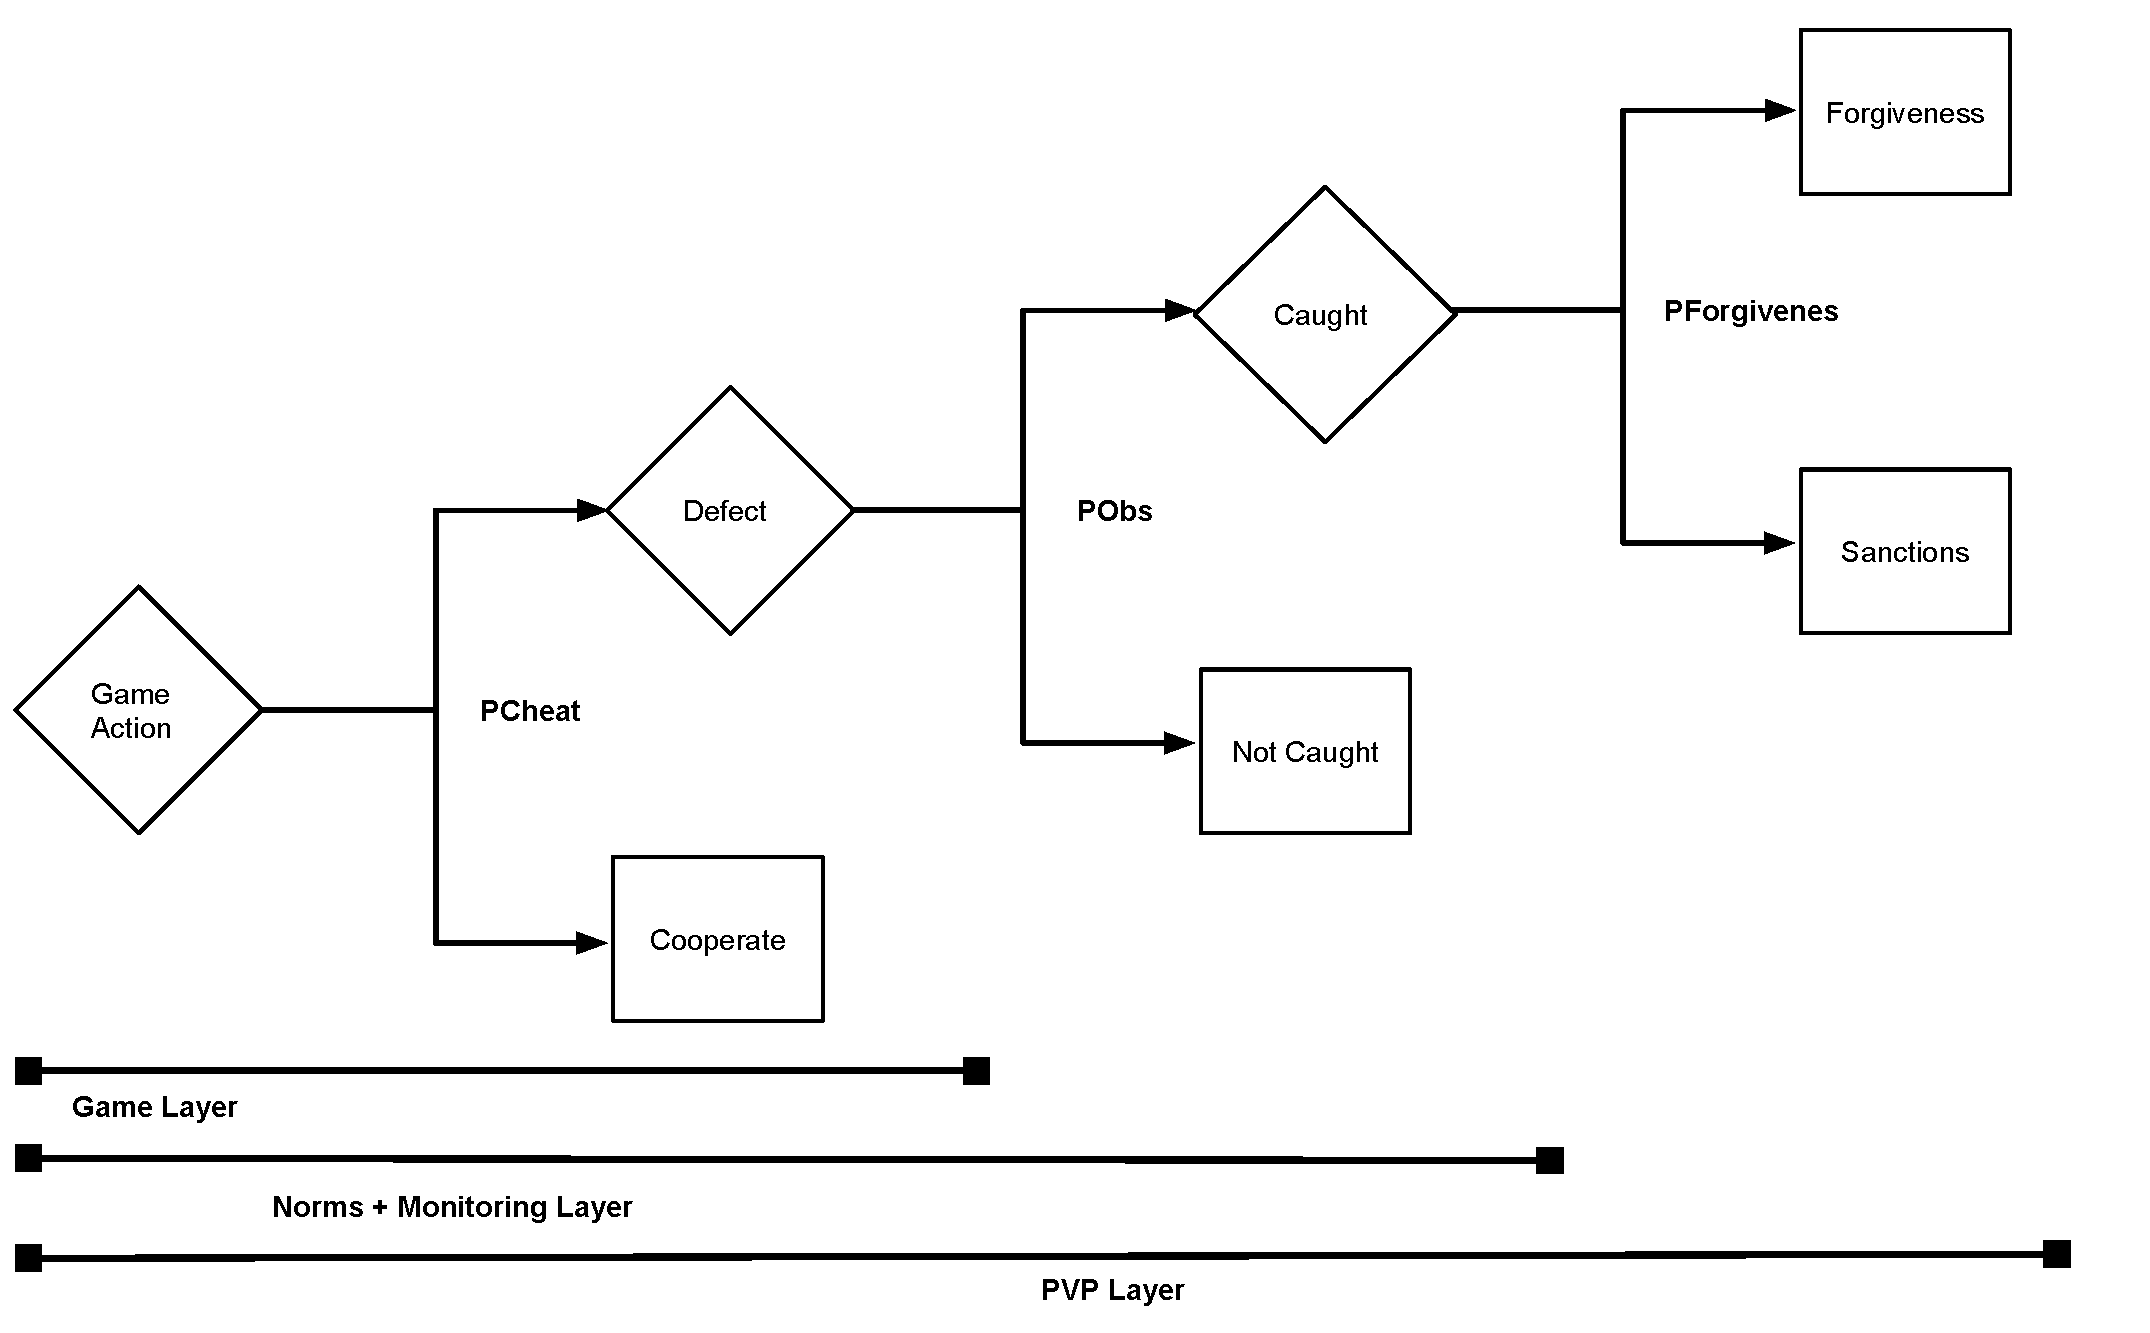
\includegraphics[width=1.0\linewidth]{img/punishflow.pdf} 
  %\caption{Model's scheme of decisions. Based on diagram presented in \cite{axelrod_evolutionary_1986}.}
  \label{fig:flow}
\end{figure}
\begin{itemize}
\item Common-pool resource management scenario
\item Linear Public Goods \textbf{game} ($LPG'$)
\begin{itemize}
    \item Agents produce and consume resources
    \item Cooperation to a common-pool is voluntary
    \item Individual resources are allocated from the common-pool
\end{itemize}
\item \textbf{Norms}:
\begin{itemize}
    \item Agents must provide all its generation to the common-pool
\end{itemize}
\item \textbf{Sanctioning system:}
\begin{itemize}
    \item Non-cooperation is liable to punishment and sanctioning
    \item Mandatory Non-repudiation: agents can't reject sanctions
    \item Selective Non-application: the issue of sanctions is optional
\end{itemize}
% \item Agents' \textbf{behavioural parameters}:
% \begin{itemize}
%     \item \textbf{PCheat:} probability of non-cooperative behaviour
%     \item \textbf{PObs:} frequency of monitoring for non-compliant events
%     \item \textbf{PForg:} probability of not issuing a sanction upon an observed non-compliant event
% \end{itemize}
\end{itemize}
\end{block}

\begin{block}{Agents' behavioural parameters}
\begin{itemize}
    \item \textbf{PCheat:} probability of non-cooperative behaviour
    \item \textbf{PObs:} frequency of monitoring for non-compliant events
    \item \textbf{PForg:} probability of not issuing a sanction upon an observed non-compliant event
\end{itemize}

\end{block}

\end{column}


%%%% Second Column
\begin{column}{.47\textwidth}


\begin{block}{Experimental Results}
\end{block}

\begin{block}{A - PVP is cost effective}


\begin{columns}[T]
\begin{column}{.7\textwidth}
\begin{figure}%{l}{0.5\linewidth}
  \centering
  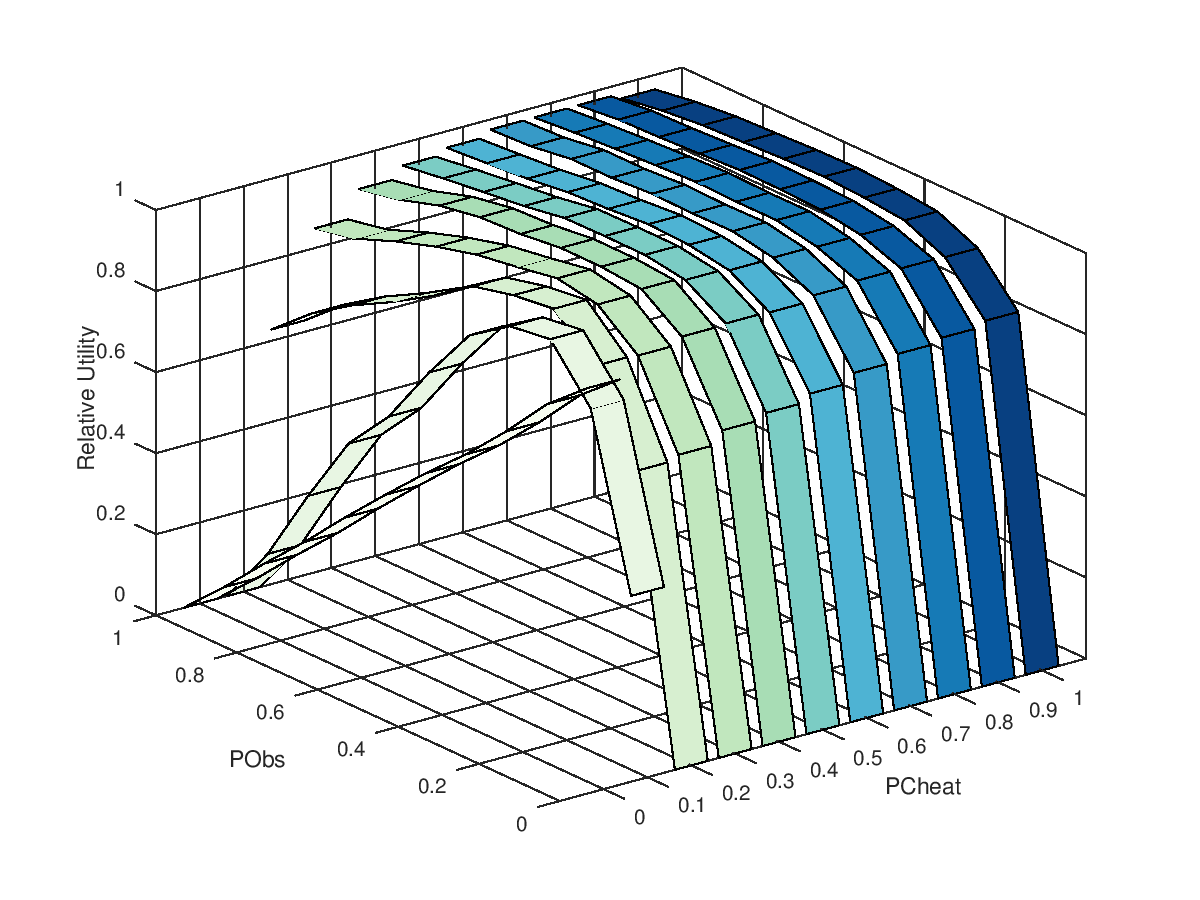
\includegraphics[width=1.0\linewidth]{img/exp1a.png}%
%  \caption{Relative utility of compliant agents for different combinations of
%    $PObs$ and $PCheat$. Note that, depending on the amount of non-compliance,
%    the increase of monitoring has small effect on the utility.}
  \label{respobs}
\end{figure}

\end{column}
\begin{column}{.3\textwidth}

If monitoring has costs, depending on the levels of non-compliance ($PCheat$), increasing the monitoring frequency ($PObs$) has small or negative effect on general utility.

\end{column}
\end{columns}
\end{block}


\begin{block}{B - PVP is tolerant and resilient to accidents}

\begin{columns}[T]
\begin{column}{.7\textwidth}

\begin{figure}
  \centering
  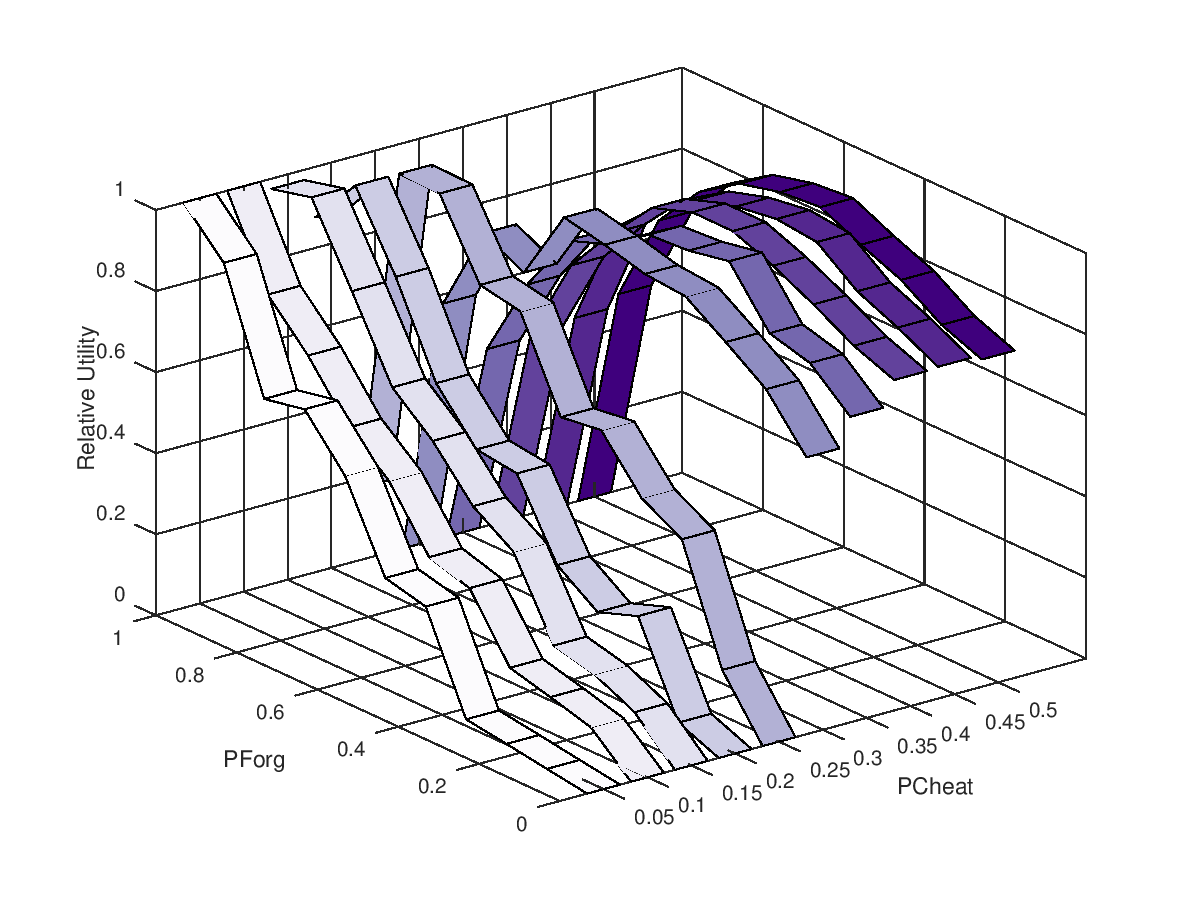
\includegraphics[width=1.0\linewidth]{img/exp1b.png}%
%  \caption{Relative utility for different combinations of $PForg$ and $PCheat$.
%    Note that especially in scenarios with low non-compliance, higher utility is
%    achieved by letting eventual non-compliant agents participate in the game,
%    than excluding them through sanctioning.}
    \label{respforg}
  \end{figure}

\end{column}
\begin{column}{.3\textwidth}


When levels of non-compliance ($PForg$) are low, punishment can be counter-productive, as it might not distinguish accidents and might exclude collaborative agents.

% Relative utility for different combinations of $PForg$ and $PCheat$.
% Note that especially in scenarios with low non-compliance, higher utility is
% achieved by letting eventual non-compliant agents participate of the game,
% than excluding them through sanctioning.

\end{column}
\end{columns}
\end{block}


\begin{block}{C - PVP is adaptable to different scenarios and behaviours}

\begin{columns}[c]
\begin{column}{.7\textwidth}

\begin{figure}
  \centering
  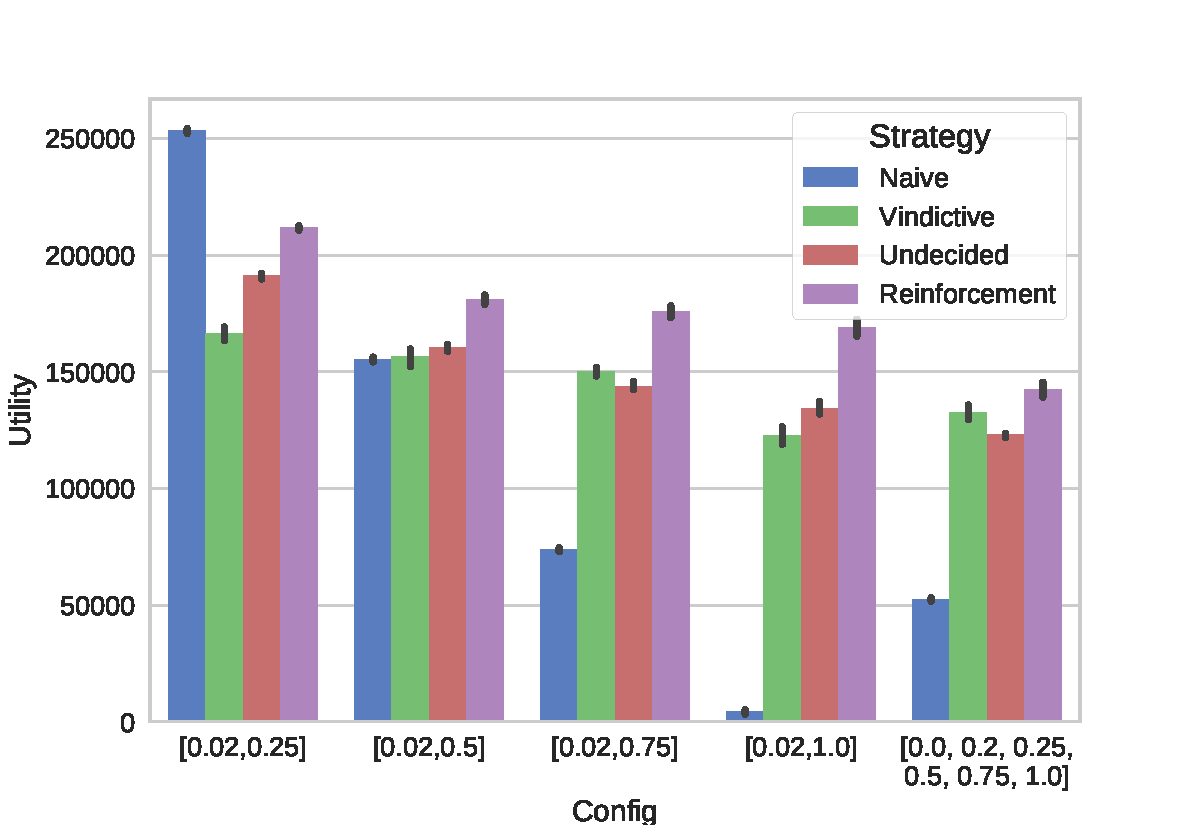
\includegraphics[width=1.1\linewidth]{img/exp2.pdf}%
%  \caption{Comparison of utility from different strategies, for various
%    configurations of population. Each configuration label shows the different
%    values of $PCheat$  among the players population. The reinforcement strategy is
%    able to achieve the best results overall in different categories.}
  \label{respvar}
\end{figure}

\end{column}
\begin{column}{.3\textwidth}

Compared to fixed policy strategies, flexible strategy (reinforcement, in graph) is able to achieve overall better results, for different scenarios of non-compliance.

\end{column}
\end{columns}
\end{block}


\begin{block}{D - PVP as a tool for justice perception}

\begin{columns}[c]
\begin{column}{.7\textwidth}

\begin{figure}
  \centering
  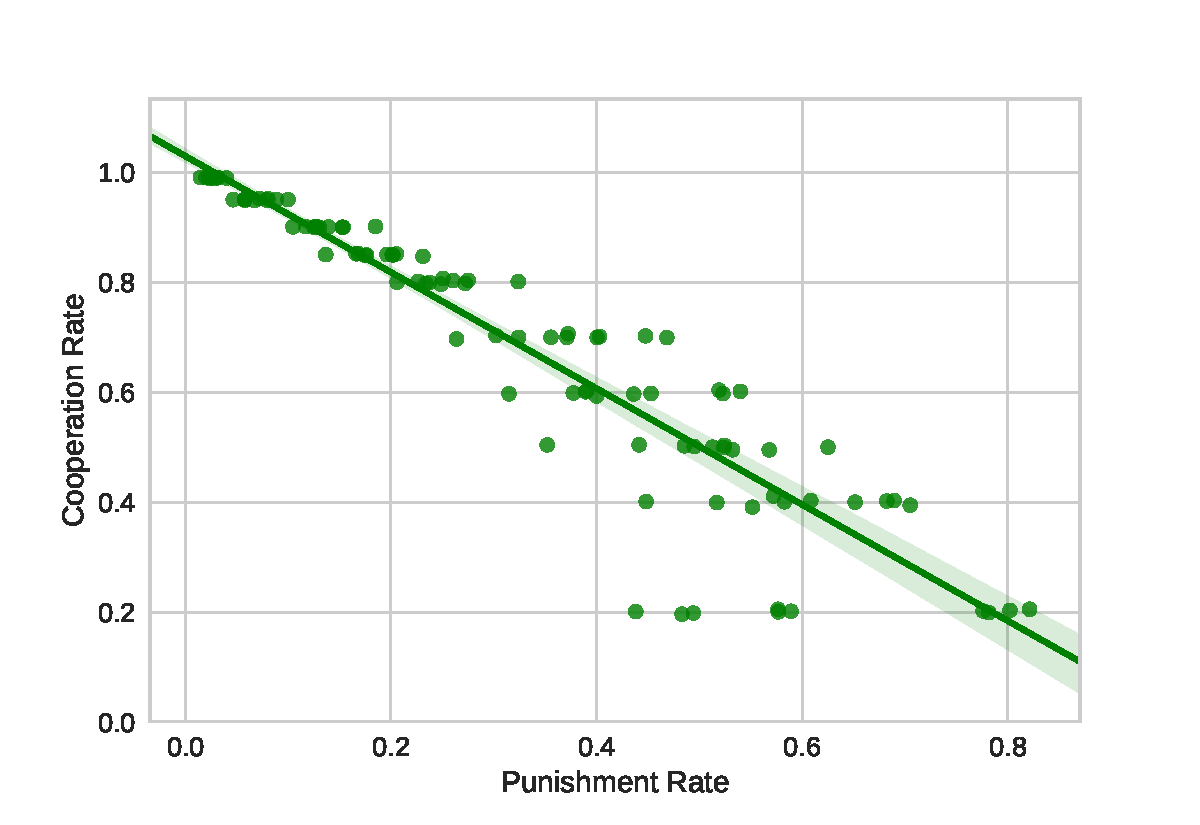
\includegraphics[width=1.1\linewidth]{img/exp3.pdf}%
%  \caption{Relationship between cooperation rate and punishment rate. The
%    inverse correlation shows that agents with high levels of cooperation
%    receive proportionally less sanctions than the ones who do not cooperate as often.}
  \label{resppercep}
\end{figure}

\end{column}
\begin{column}{.3\textwidth}

% In scenarios where $PObs$ and $PForg$ are learned through reinforcement and observation, 

In scenarios where PVP is learned and exercised, agents with high levels of cooperation receive proportionally less sanctions than the ones who do not cooperate as often.


\end{column}
\end{columns}
\end{block}



\end{column}
\end{columns}


\end{frame}
\end{document}